\chapter{Dark matter}
\label{ch:dm}
%P1, the Standard Model -> dark matter
\par As mentioned in Chapter~\ref{ch:sm}, about one quarter of the total mass-energy in the universe is dark matter. No known particle that can account for the dark matter in the universe, and single-particle model is disfavored. Therefore, current models consider dark matter as a whole sector of new particles, instead of the existence of a single new type of particle.

%P2, chapter structure
\par This chapter is organized as follows: the astrophysical measurements establishing of dark matter and its particle physics explanation are discussed in Section~\ref{sec:dms1}. In Section~\ref{sec:dms2}, dark matter as a microscopic particle, Weakly Interacting Massive Particle, is described. Finally, Section~\ref{sec:dms3} outlines how dark matter particles might be produced by particle colliders and what signatures they might generate.

\section{Dark matter: From astrophysics to particle physics}
\label{sec:dms1}

%P1,
\par The concept of dark matter originates from physical observations. Multiple astrophysical observations at different distance scales prove the existence of invisible matter in the universe. The concept of dark matter was formally brought up by Jacobus Kapteyn in the studies of the velocity distribution of stars in nearby galaxies~\cite{Kapteyn:1922zz}. These studies showed that the amount of visible matter from stars and interstellar gas near the solar system was not sufficient to explain the motions of the stars perpendicular to the Milky Way disk. The visible matter doesn't provide enough gravitational force attraction which suggests the existence of the unobserved matter. Another proof on galactic scales is the motion of the Coma galaxy cluster observations by Fritz Zwicky in 1933~\cite{Zwicky:1933gu}, which suggested a large contribution to the gravitational forces that is not visible.

\par On galactic scales, the most convincing evidence is the direct observation of the rotation curves of galaxies, which shows the orbital velocities of stars and gas inside a galaxy as a function of their distance from the galactic center. According to the Newtonian theory of gravity, the rotation velocity, $v(r) \propto \frac{1}{\sqrt{r}}$, which is in contrast with observed curve in Fig.~\ref{fig:rotation}. It is the discrepancy between the observed and expected velocities that has led to the belief that some form of dark matter must exist. And this suggests the existence of a dark (invisible) halo with $M(r) \propto r$ and $\rho \propto \frac{1}{r^2}$.

\begin{figure}[htbp]
    \centering
    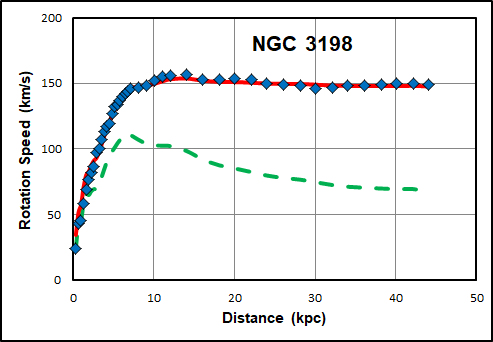
\includegraphics[width=0.8\textwidth]{chapters/c2/figures/ngc3198_sparc.jpg}
    \caption{The rotation curve for spiral galaxy NGC 3198. The blue diamonds are the observations and reveal the almost flat-like nature of the curve in the outer regions of the galaxy. The dashed green line is the curve for Newtonian gravity. It shows that the rotational velocity should decrease with distance from the galaxy center. The solid red line through the data points is the curve obtained by assuming a simple Gaussian energy scale variation and a simple Gaussian density distribution for the galaxy.}
    \label{fig:rotation}
\end{figure}

\par The Cosmic Microwave Background (CMB), is electromagnetic radiation remnant from an early stage of the universe, also known as ``relic radiation''. On the cosmological scale, not only does CMB show evidence of dark matter, in the context of specific models it also quantifies the amount of dark matter in the Universe. Experiments measure the power spectrum of the CMB. Now the Lambda-CDM model best fits the observation data, giving values for the density of baryonic matter, dark matter, and Dark Energy.

\par Hot dark matter (HDM) theory~\cite{Zeldovich:1982zz} was established in 1980 by Zeldovich's team. HDM assumes that the light neutrinos make up the majority of the dark matter. It is natural to assume that the dark matter is the weakly coupled particle that already exists in the Standard Model. However, the conventional neutrino-dominated picture is ruled out by early universe simulation studies in 1983~\cite{White:1984yj}. Afterwards, scientists realized that only with a slow-paced particle, so-called ``cold'' dark matter, the diffusion of small scale fluctuation can be prevented. The early universe structure can be formed on all scales is consistent with this astrophysical observations. Therefore, the cold dark matter theory (CDM theory)~\cite{PhysRevLett.48.223} was established in 1983 to explain the cosmic microwave background observation result. Nowadays, as an important part of the standard cosmological model (Lambda-CDM theory), the concept of cold dark matter is widely accepted. 

\section{Weakly Interacting Massive Particles}
\label{sec:dms2}
%P1, why WIMPs
\par Although the existence of cold dark matter around galaxies and clusters is supported by cosmological observation, scientists still have poor knowledge regarding to the nature of cold dark matter is. Under the assumption it is a particle, the observation of cold dark matter indicates the existence of weakly interacting particles. The density fluctuations and the small scale fluctuations indicate the mass of cold dark matter candidate can not be small. Therefore, WIMPs - weakly interacting massive particles, become one of the best candidate particles to characterize the feature of cold dark matter.

%P2, WIMPs in beyond the Standard Models
\par WIMP masses range from a few~\GeV~to $\mathcal{O}$(~\TeV), to match the observed relic density from the CMB analysis. Both popular beyond SM models Supersymmetry (SUSY) and Extra-dimensions, there are WIMP candidates of DM particles. The electrically neutral lightest supersymmetric particle (LSP) predicted in an R-parity conserving scenario of supersymmetric extension of the Standard Model is an ideal candidates for dark matter. Among all possible choices, the most promising one is the lightest neutralino, which is the lightest state of the mixtures of neutral electroweak gauginos and the neutral higgsinos~\cite{Feng:2010gw}. Similarly to the phenomenology of SUSY, in universal extra dimensions (UED) models, each SM particle is accompanied by a partner particle at the first Kaluza-Klein (KK) mode level. Also, UED models preserve a geometric parity (KK parity). The lightest partner state (which in UED is the partner of the $U(1)_Y$ gauge boson) is a good dark matter candidate which can yield the observed dark matter relic density~\cite{Servant:2002aq}.

\section{Searches for dark matter in collider experiments}
\label{sec:dms3}
%P1, experimental method to search dark matter
\par Dark matter is observed through its gravitational interactions in the universe. To explore its potential particle properties, several complementary detection methods are used~\cite{Undagoitia:2015gya}: 
\begin{itemize}
  \item \textbf{Direct detection}: Direct detection is focuses on recoils of nuclei with few keV induced by interactions with dark matter particles propagating through the solar system.
  \item \textbf{Indirect detection}: Indirect detection searches for astrophysical dark matter signals from annihilation products, usually using cosmic rays.
  \item \textbf{Production at colliders}: Production at colliders, as its name suggests, looks for WIMPs in collision data. WIMPs can be detected indirectly as missing energy and momentum that escapes the detectors.
\end{itemize}

%P2, search dark matter in collider experiment
\par In the rest of this thesis, only the ``Production at collider'' approach will be considered. Several beyond the Standard Model models that have dark matter candidates will be described in the rest of this section. These models are the search target and will be used to interpret the collision data in statistical manner.

\subsection{Effective field theory}
%P1, why EFT
Before we dive into specific particle physics models, some generic principles need to be illustrated. The first concept is effective field theory. An effective field theory is an approximation for an underlying physical theory, for example quantum field theory. Assuming that all the current physical observations can be explained under one single physics theory. However, since this “theory of everything” is supposed to explain the experiment at all energy scales, the physical observables are always resulted in infinite under the quantum field theory framework. Furthermore, the important features of the known physics, namely the Standard Model, are not guaranteed to be extendable with higher energy scale. Therefore, the ultraviolet energy cut-off is needed for quantum field theory based particle physics model to guarantee the model itself renormalizable. The effective field theory~\cite{Pich:1998xt} is designed to resolve this issue.

%P2, what is EFT
\begin{figure}[htbp]
    \centering
    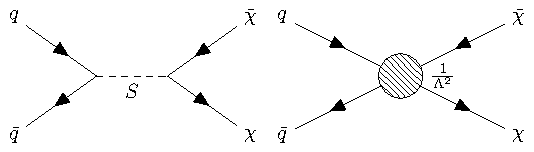
\includegraphics[width=0.8\textwidth]{chapters/c2/figures/eft-feyn-diagram}
    \caption{Left: an s-channel Feynman diagram of the interaction between quarks and dark matter candidates via a scalar mediator. Right: the corresponding effective field theory contact interaction.}
    \label{fig:c2eftfeyndiagram}
\end{figure}

In the context of particle physics, effective field theories are simplifications of the complete quantum field theories where the mass of the interaction mediator is large enough with respect to the momentum exchange of a physical process. Therefore, an s-channel process can be replaced by a contact operator as demonstrated in Fig.~\ref{fig:c2eftfeyndiagram}. In Fig.~\ref{fig:c2eftfeyndiagram}, a new scalar mediator, labeled S, is introduced to couple with both the Standard Model quarks and a dark matter candidate. The Lagrangian of this simple model is~\ref{eq:c2eftl}:

\begin{equation}
  L = \frac{1}{2}M^{2}S^{2}-g_{q}q\bar{q}S-g_{\chi}\chi\bar{\chi}S,
  \label{eq:c2eftl}
\end{equation}

where M is the mass of newly introduced scalar, $g_{\chi}$ is the coupling strength between the scalar mediator and dark matter candidates, and $g_{q}$ is the coupling constant between the scalar mediator and the Standard Model quarks. The knowledge of the quantum field theory tells us that the s-channel cross section is proportional to the factor $\frac{1}{Q_{tr}^{2}-M^{2}}$, where $Q_{tr}$ is the momentum transfer of the process. Using Taylor expansion, this factor can be expanded in powers of $\frac{Q_{tr}}{M}$: 

\begin{equation}
  \frac{1}{Q^{2}_{tr}-M^{2}} = -\frac{1}{M^{2}}(1+\frac{Q^{2}_{tr}}{M^{2}}+\mathcal{O}(\frac{Q^{4}_{tr}}{M^{4}}))
  \label{eq:c2taylorexp}
\end{equation}

If $Q_{tr} \ll M$, the propagator term can be simplified as $-\frac{1}{M^2}$. Therefore, the interaction vertices of the s-channel collapse into a contact point: $O_{s}=\frac{g_{q}g_{\chi}}{M^{2}}\chi\bar{\chi}q\bar{q}$, where $\Lambda=\frac{g_{q}g_{\chi}}{M^{2}}$ can be viewed as the mass scale of the effective field theory. Given the condition that $Q_{tr} \ll M$, the constraint of the new energy scale can be derived as~\ref{eq:c2scalelimit}:

\begin{equation}
  \Lambda \gg \frac{Q_{tr}}{\sqrt{g_{q}g_{\chi}}}
  \label{eq:c2scalelimit}
\end{equation}

Therefore, the calculation can be simplified for any process that satisfies the condition in Equation~\ref{eq:c2scalelimit}.

\subsection{The simplified model}
%P1, why simplified model
\par Although the energy scale can be limited with the effective field theory, the simulation can still be complex due to the model structure itself. For example, in the simplest supersymmetry scenario, the Minimal Supersymmetric Standard Model, there are more than 100 free parameters. It is almost impossible to explore them all within a search for one signature. Therefore, simplified models~\cite{SimplifiedModels-Alves2012} are used.

%P2, what is simplified model
\par A simplified model describes the particles relevant to the search process only. With the help of simplified models, the complex interaction Feynnman diagram group can be trimmed into one or several tree-level diagrams that describe the signal of interest. As a result, the model calculation is simplified while its characteristics are still preserved. 

%P3
\par With the simplification of effective field theory and simplified model, several models are introduced in the rest of this section. The physical events from these models are used as search signal for the rest of this thesis.

\subsection{$Z^{\prime}$ and Two-Higgs-doublet models}
%P1, Z' model, why
\par A $Z^{\prime}$ model~\cite{He:1991qd} is one of the simplest Standard Model extensions that can have a dark matter candidate. As mentioned in Section~\ref{sec:dms2}, the dark matter candidate as fundamental particle needs to be both weakly interacting and massive. Therefore, a natural way to introduce a weakly couples particle into the Standard Model is to add a new vector boson that coupled with WIMPs. This newly added particle is a massive, neutral boson. The simplest gauge structure for this beyond the Standard Model is a U(1) extension. However, this newly added U(1) can be a derivative from more a complex symmetry, like SU(2), or $E_{6}$. This simplest extension of the Standard Model is called a $Z^{\prime}$ model.

%P2, Z' model, what
\par The $Z^\prime$ boson can couple with both the Standard Model quarks and dark matter candidates. A typical Feynnman diagram is shown in Fig.~\ref{fig:c2zprime}. However, the mass of the dark matter candidate is highly constrained by the Higgs boson mass, therefore, it is less possible to find a massive dark matter candidate within the current experiment constraints in $Z^{\prime}$ model. But mixing the $Z^{\prime}$ model with other beyond Standard Model models we can gain more room in parameter space. One of the examples is a $Z^{\prime}-2HDM$ model, a mixture of a $Z^{\prime}$ model and a Two-Higgs-doublet model.

%P3, 2HDM, why
\par Before describing the mixed model, let us summarize the features of Two-Higgs-doublet models~\cite{Branco:2011iw}, abbreviated as 2HDM. 2HDM are multiple Higgs doublet extensions of Standard Model. 2HDM models are inspired by supersymmetric models~\cite{Martin:1997ns} and Axion model~\cite{Peccei:2006as}. Therefore, 2HDMs can not only provide a dark matter candidate, but also bring enough CP violation to support baryon asymmetry universe.


%P5, Z'+2HDM
\par As mentioned, $Z^{\prime}$ and Two-Higgs-doublet models can be combined into mixed models to provide much richer phenomenological predictions. The Higgs-like field in the 2HDM is introduced into the $Z^{\prime}$ model as a dark matter mediator. As a result, the mixture $Z^{\prime}+2HDM$ model~\cite{Berlin:2014cfa} can provide sufficiently massive dark matter candidate while respecting experimental data constraints with its larger parameter space.

%P6, Higgs bb channel in 2HDM and Z'+2HDM
\begin{figure}[htbp]
    \centering
    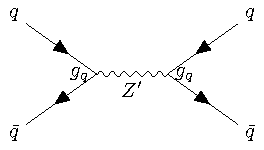
\includegraphics[width=0.5\textwidth]{chapters/c2/figures/z-prime}
    \caption{Feynman diagram of the interaction between Standard Model quarks and a $Z^{\prime}$ boson.}
    \label{fig:c2zprime}
\end{figure}

\begin{figure}[htbp]
    \centering
    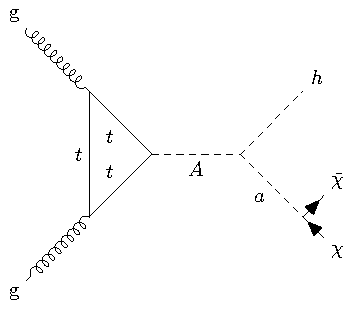
\includegraphics[width=0.5\textwidth]{chapters/c2/figures/two-higgs}
    \caption{The Feynman diagram of the interaction between the Standard Model quarks and $Z^{\prime}$ boson.}
    \label{fig:twohiggs}
\end{figure}

\begin{figure}[htbp]
    \centering
    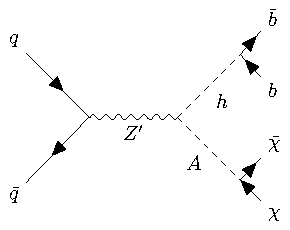
\includegraphics[width=0.5\textwidth]{chapters/c2/figures/z-prime-2hdm}
    \caption{The Feynman diagram of $b\bar{b}$ decayed Higgs channel in $Z^{\prime}+2HDM$.}
    \label{fig:c2zprime2hdm}
\end{figure}


\par With the discovery of the Higgs boson, the study of Higgs properties becomes the frontier of particle physics. The Higgs boson is widely used as a physics object, like the top quark after 1995, in new physics searches. Given our limited knowledge of the Higgs boson, it is quite possible that is couples dark matter sector in some way. Among all the Higgs decay channels, Higgs~$\rightarrow b\bar{b}$ is the one with the largest branching ratio. Therefore, it is natural for experimentalists to search dark matter candidates produced in association with the Higgs boson in the channel with large missing transverse momentum and Higgs~$\rightarrow b\bar{b}$ decay as its signature. The Feynman diagram of Higgs~$\rightarrow b\bar{b}$ channel is shown in Fig.~\ref{fig:twohiggs} for a Two-Higgs-doublet model, and in Fig.~\ref{fig:c2zprime2hdm} for the $Z^{\prime}+2HDM$. Both are studied as the signal in the rest of this thesis.
